\section{Hardware Search and Speedup Analysis}
\label{app:solver}\label{app:deficit}
\suppressfloats[t]

Wall-clock time decomposition and search acceleration results are presented in Figure~\ref{fig:wallclock} and Section~\ref{sec:experiments}.

% retained but disabled: legacy wall-clock figure (static / V0 / V1)
% \begin{figure}[t]
%     \centering
% 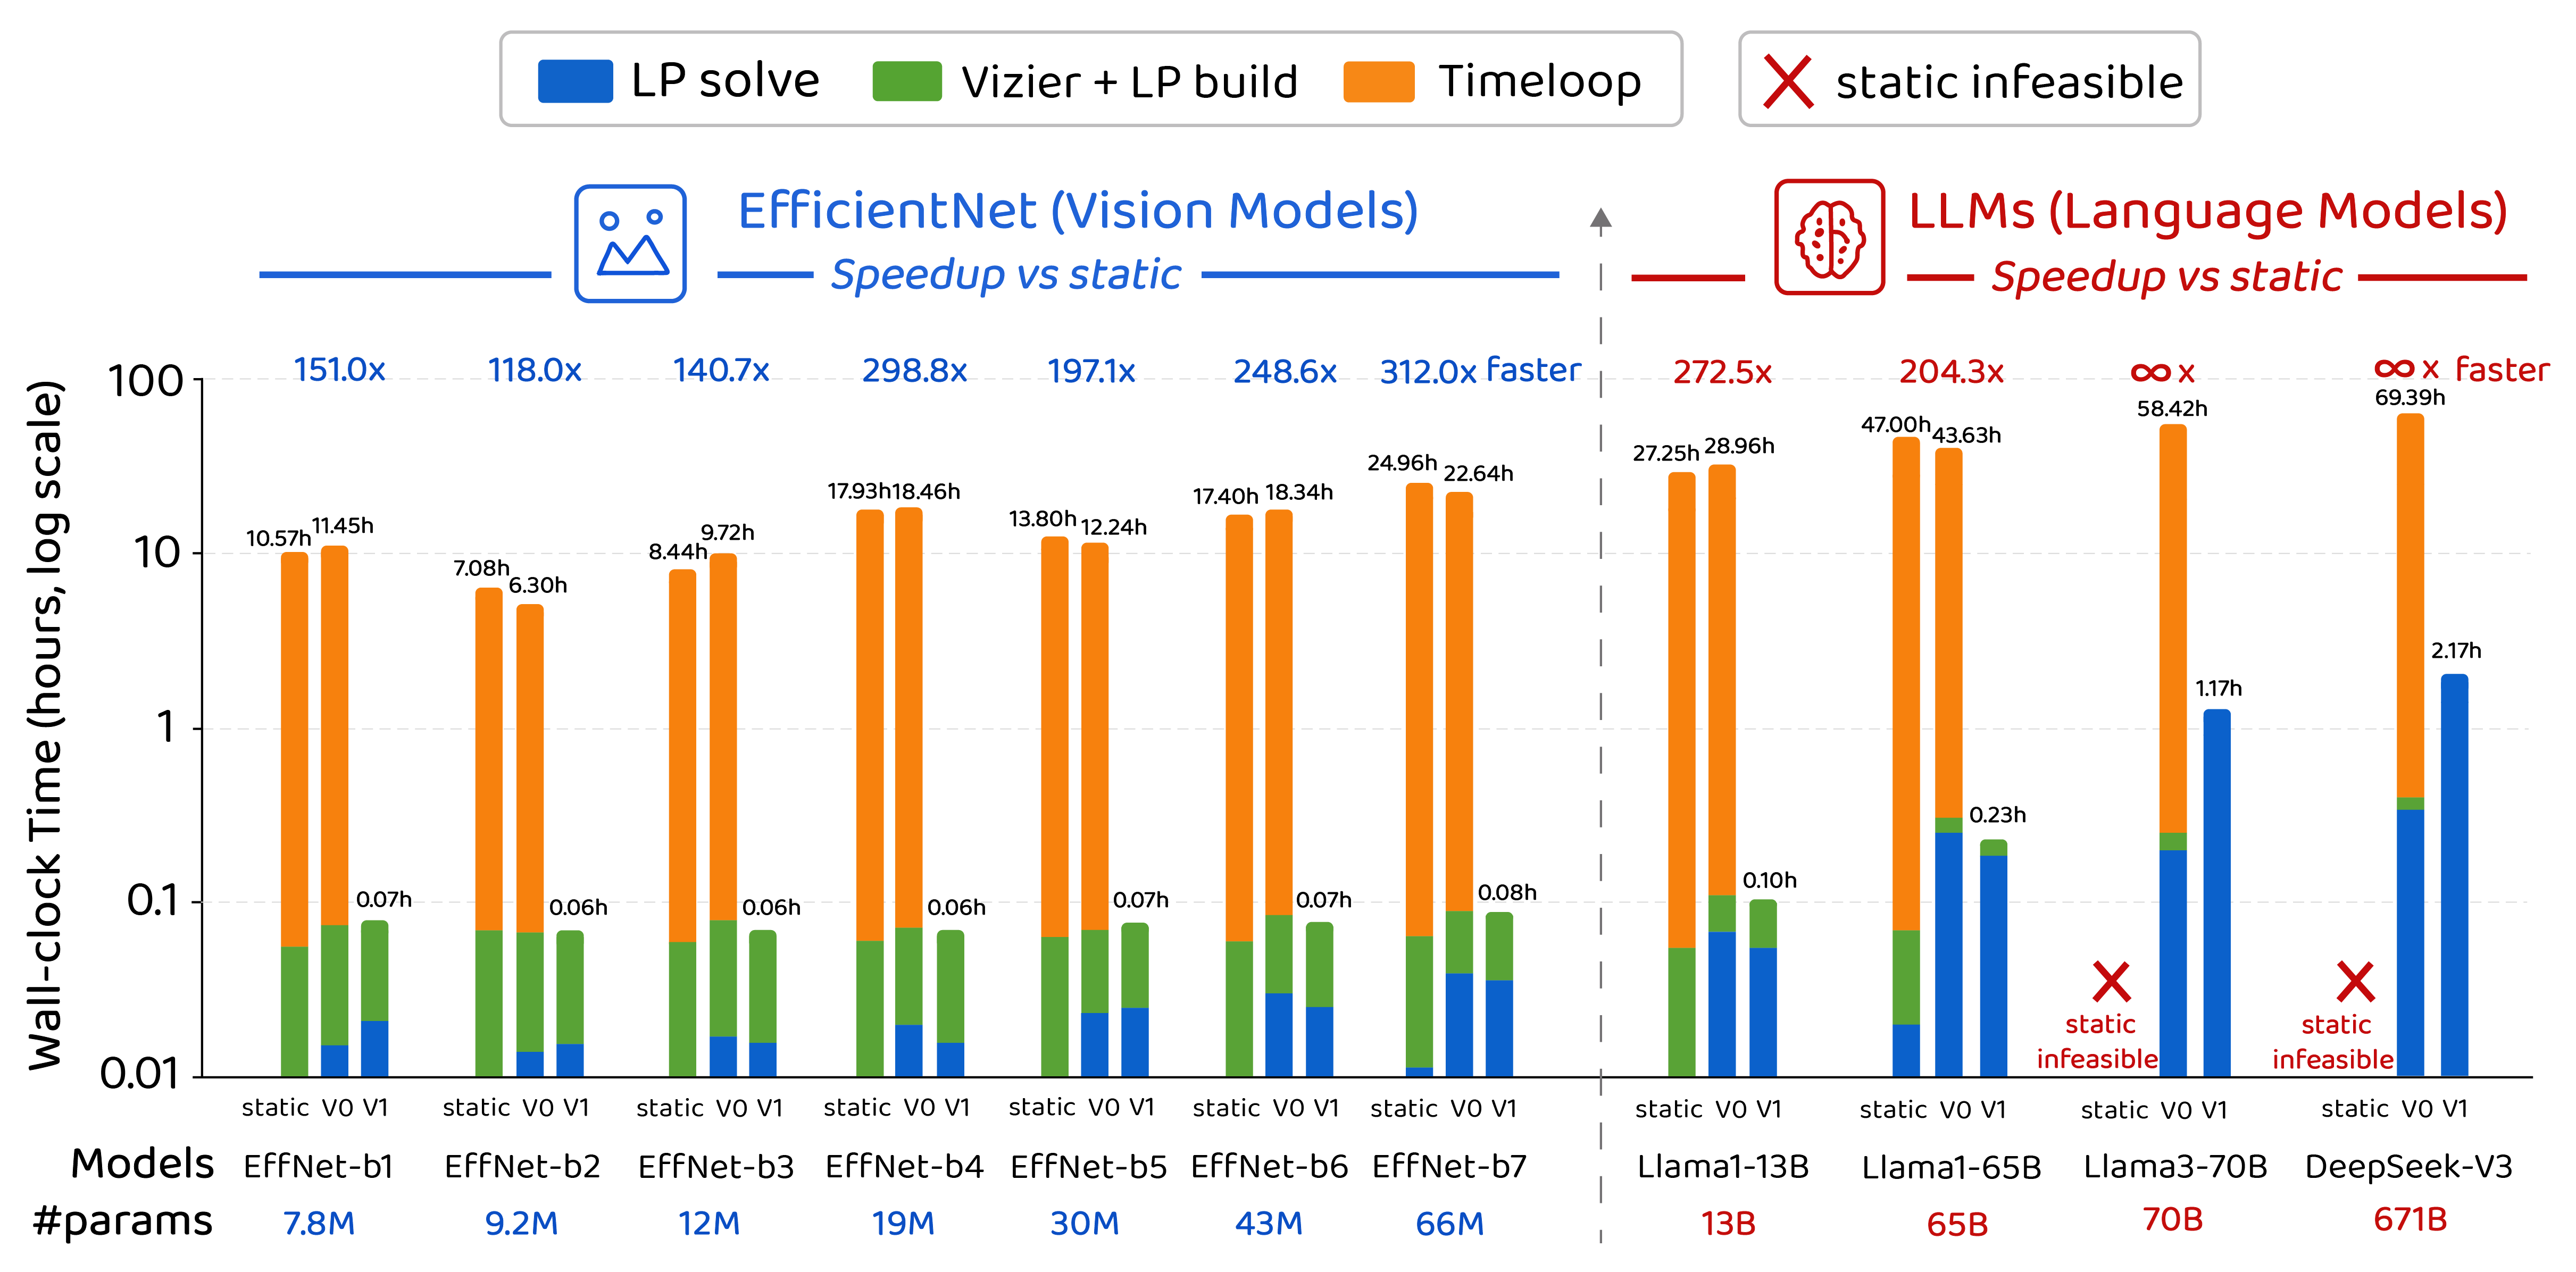
\includegraphics[width=1.0\linewidth]{fig3/wallclock_new_v6.png}
% \caption{Wall-clock time decomposition and performance acceleration across formulations: CHEETAH's internalized tiling eliminates the Timeloop bottleneck, achieving up to 100--300$\times$ faster search than the classical static method. Upper bars show wall-clock hours (log scale), annotations show speedup vs.\ static.}
% \label{fig:wallclock}
% \end{figure}

\begin{figure}[t]
    \centering
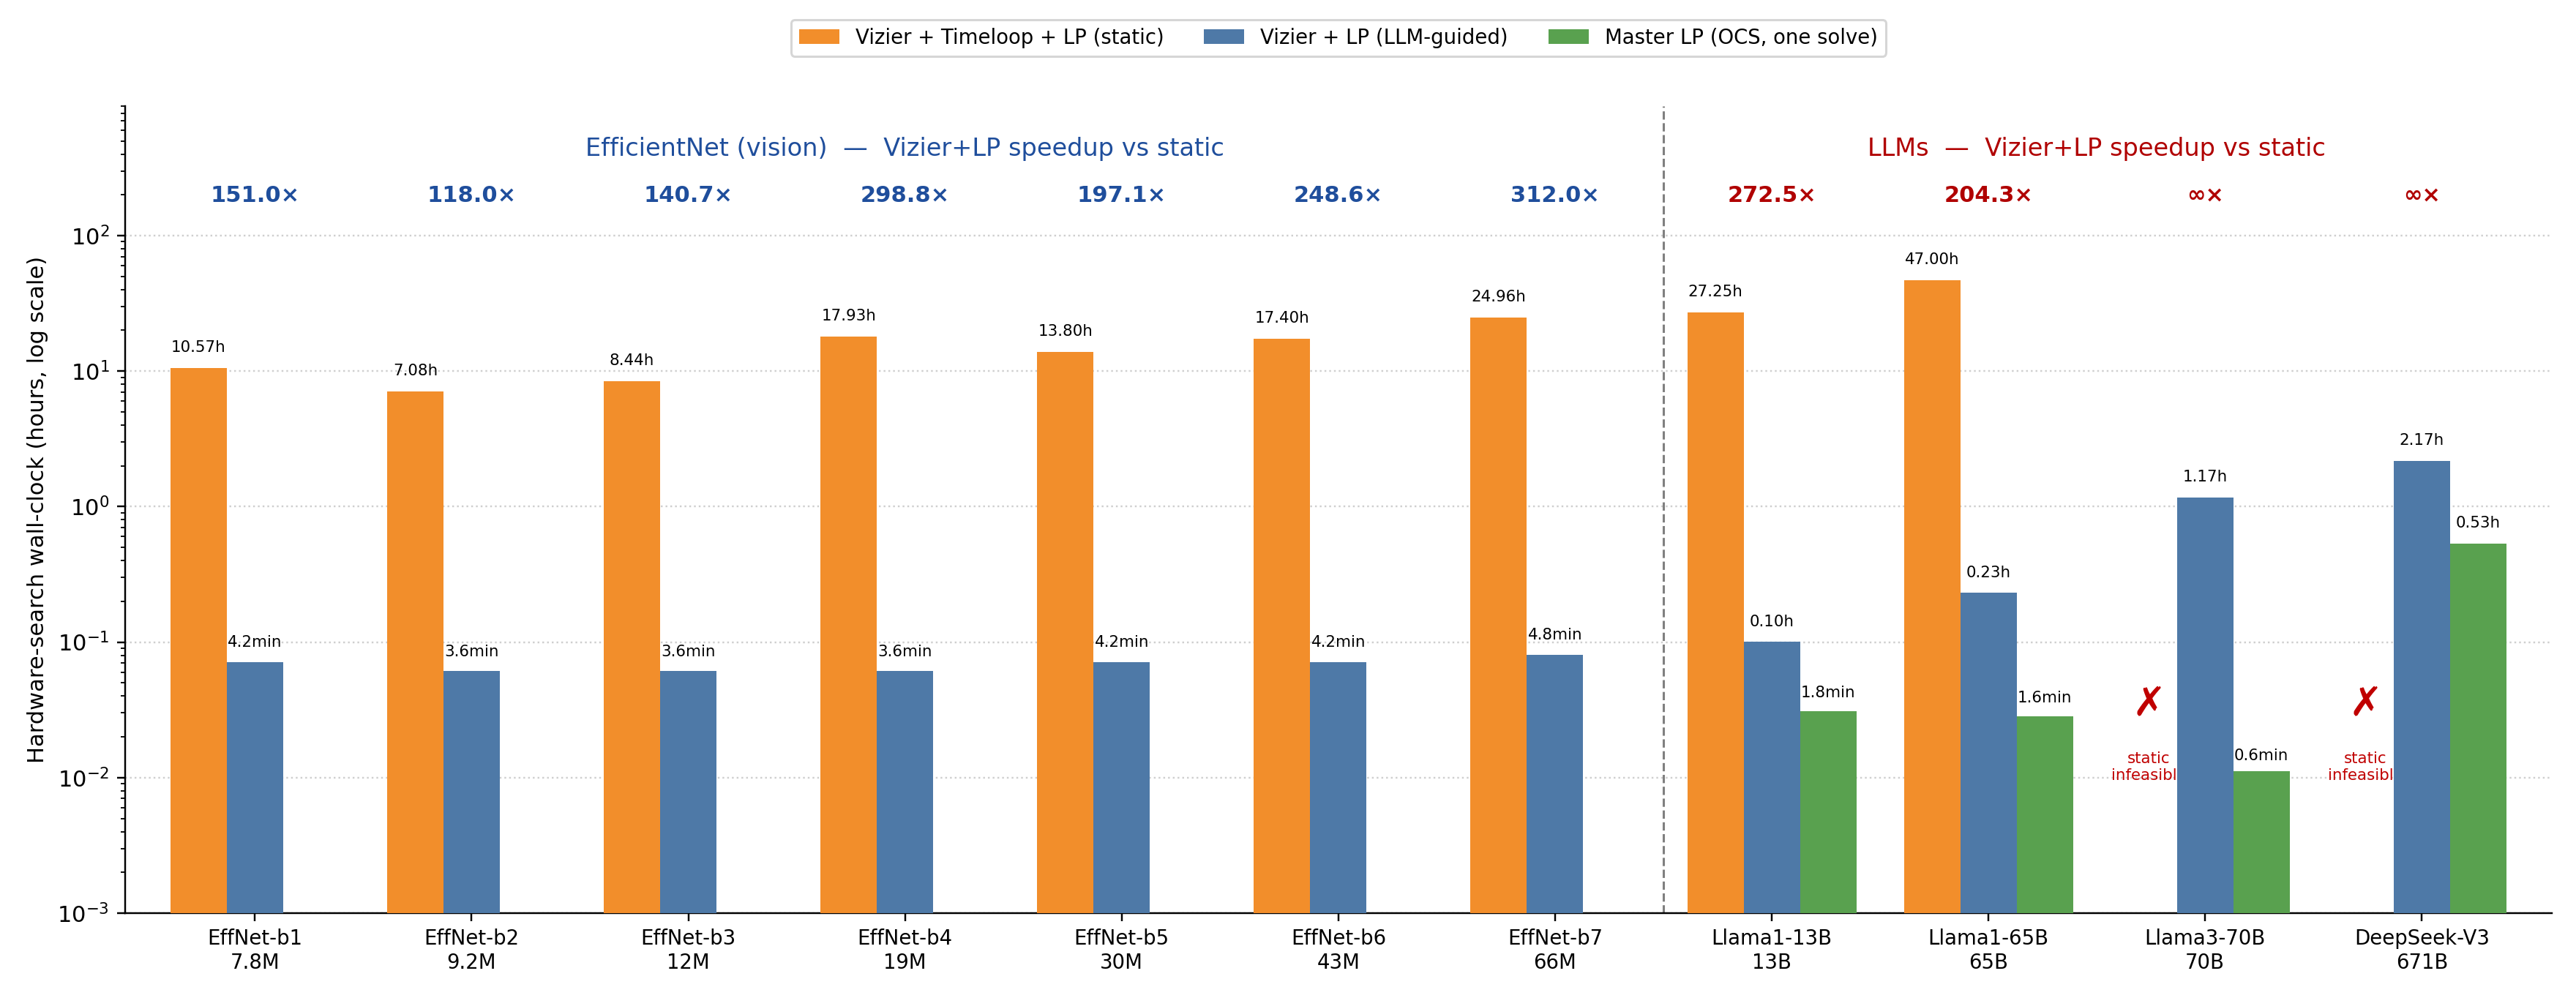
\includegraphics[width=1.0\linewidth]{fig3/wallclock_three_methods_v1.png}
\caption{Hardware-search wall-clock across three formulations, log scale. Vizier+Timeloop+LP is the static method with a mapper call inside every trial, and Vizier+LP is the LLM-guided joint-tile formulation with cached implementation coefficients. Both are 50-trial searches on one H100, and the annotations give the Vizier+LP speedup over the static method. The master LP column is the summed wall-clock of the OCS solve stages that produced the retained LLM decoder designs, with the whole-chip alternatives inside the finite program, measured on an A100 host, split into joint and hardware-screen solves, fixed-chip controls, and branch and bound with certificates. The 50-trial bars split into Timeloop, Vizier plus LP build, and LP solve time. The master LP column is a different experiment with a different trial structure, and the vision designs have no such column because they are analytical recoveries with no new solver call. Red crosses mark workloads on which the static method is infeasible.}
\label{fig:wallclock}
\end{figure}



\subsection{Hardware and Vizier Search}\label{app:vizier_search}

The prefill co-design search used 16 NVIDIA H100 GPUs, each with 80 GB of VRAM, and Vizier for hardware search following the experimental conventions of \citet{zhang_fast}.
Table~\ref{tab:vizier_search_space} records that campaign's parameter groups; Figure~\ref{fig:pipeline} depicts its accelerator template.
The native full-inference extension is solved with OCS (Section~\ref{sec:ocs}) with a separate finite hardware-search path.
It is not an all-H100/Vizier experiment.

A Processing Element (PE) is a repeated compute tile in an accelerator template.
The datapath can be modeled as a grid of PEs connected by a mesh on-chip network.
PE systolic arrays perform a matrix-vector multiply each cycle.
Vector and scalar MACs are modeled by setting systolic array X and Y dimensions to 1.
PEs also contain a VPU for non-MAC vector ops.
L2 and Global Memory structures are optional. 

\begin{figure}[ht!]
    \centering
    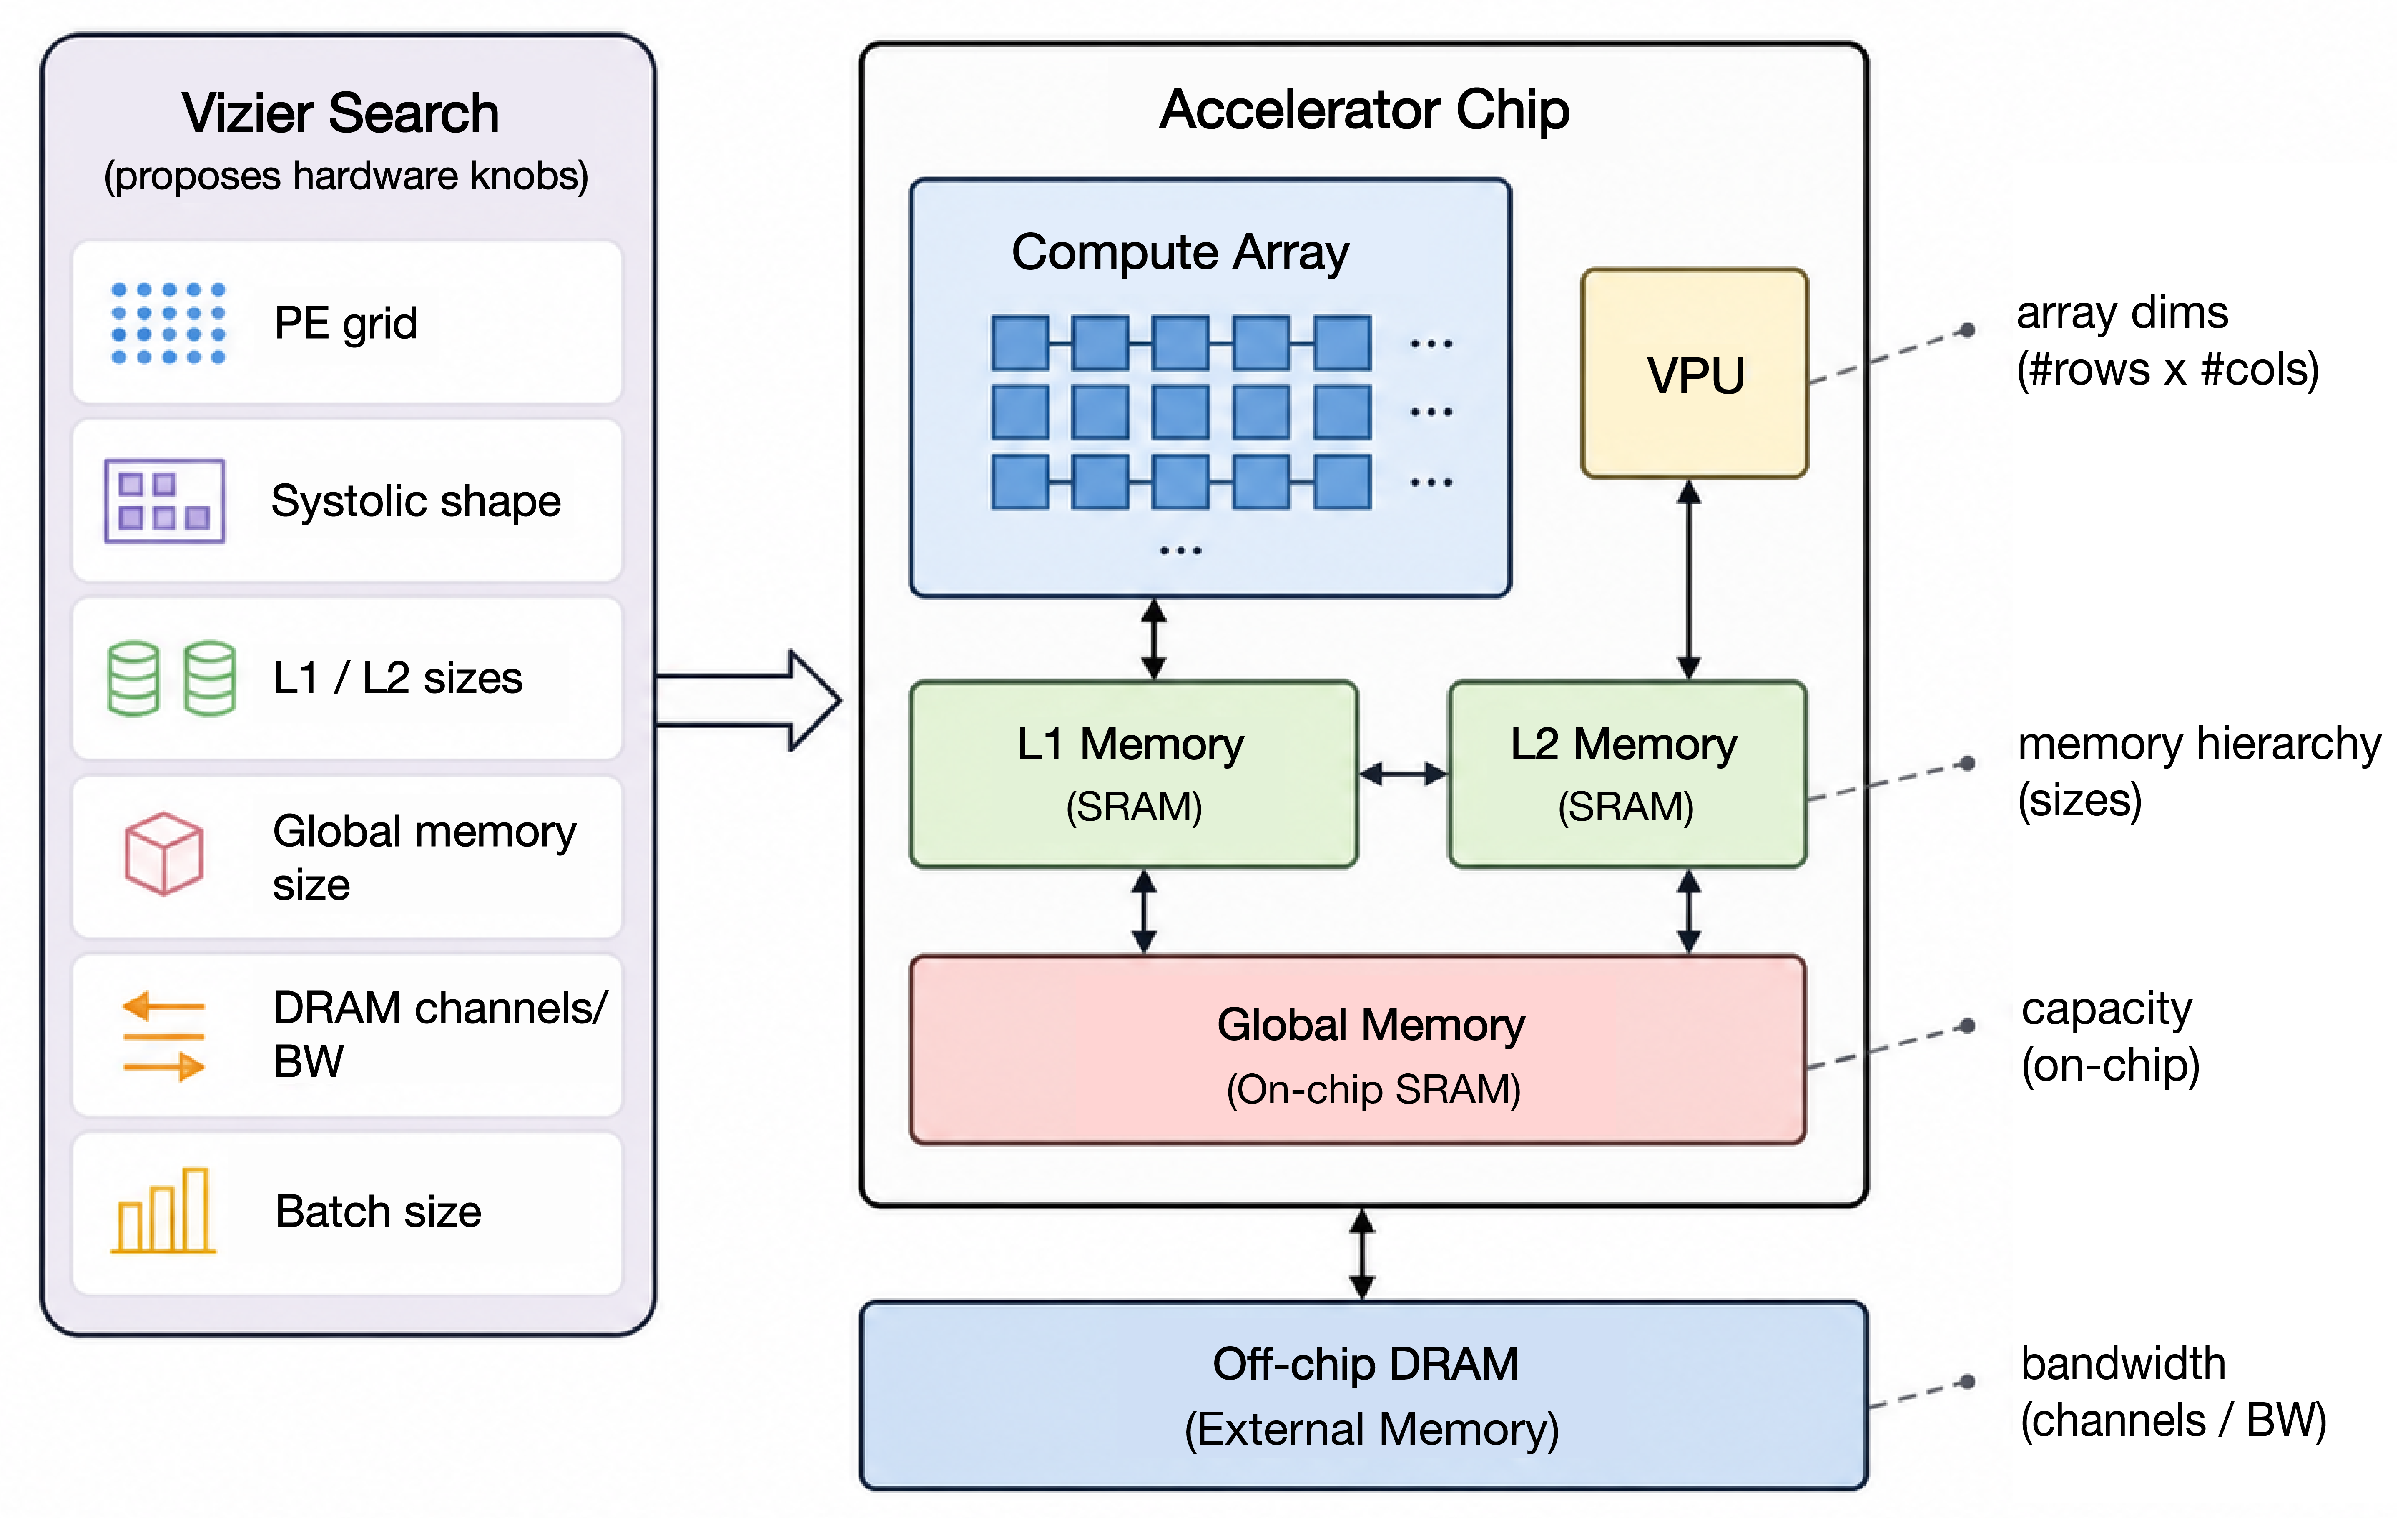
\includegraphics[width=0.7\linewidth]{figs/hardware_layout_v4.png}
    \caption{The accelerator datapath configuration. Processing elements (PEs) are arranged in a grid connected by a mesh network. Each PE contains a systolic array for matrix operations, a vector processing unit (VPU) for non-MAC operations, and private or shared L1/L2 memory. A Global Memory serves as the on-chip scratchpad shared across all PEs.}
    \label{fig:pipeline}
\end{figure}
\label{app:vizier}


\begin{table}[h]
\centering
\caption{Vizier search parameter groups and ranges: initial small search vs.\ expanded joint-tile-wide search.}
\label{tab:vizier_search_space}
\resizebox{\textwidth}{!}{%
\begin{tabular}{llll}
\toprule
\textbf{Group} & \textbf{Parameter} & \textbf{Small (initial)} & \textbf{LLM-joint-tile-wide} \\
\midrule
\multirow{16}{*}{\textbf{A: Hardware datapath (16 params)}}
 & \texttt{PEs\_x\_dim}                & pow2 in $\mathbf{4 \ldots 32}$                          & pow2 in $\mathbf{1 \ldots 256}$                        \\
 & \texttt{PEs\_y\_dim}                & pow2 in $\mathbf{4 \ldots 32}$                          & pow2 in $\mathbf{1 \ldots 256}$                        \\
 & \texttt{Systolic\_array\_x}         & pow2 in $\mathbf{4 \ldots 32}$                          & pow2 in $\mathbf{4 \ldots 128}$                        \\
 & \texttt{Systolic\_array\_y}         & pow2 in $\mathbf{4 \ldots 32}$                          & pow2 in $\mathbf{4 \ldots 128}$                        \\
 & \texttt{Vector\_unit\_multiplier}   & pow2 $1 \ldots 16$                                      & pow2 $1 \ldots 16$                                     \\
 & \texttt{L1\_buffer\_config}         & \{Private, Shared\}                                     & \{Private, Shared\}                                    \\
 & \texttt{L1\_input\_buffer\_size}    & pow2 $\mathbf{1\,\text{KB} \ldots 4\,\text{MB}}$        & pow2 $\mathbf{1\,\text{KB} \ldots 1\,\text{MB}}$       \\
 & \texttt{L1\_weight\_buffer\_size}   & pow2 $\mathbf{1\,\text{KB} \ldots 4\,\text{MB}}$        & pow2 $\mathbf{1\,\text{KB} \ldots 1\,\text{MB}}$       \\
 & \texttt{L1\_output\_buffer\_size}   & pow2 $\mathbf{1\,\text{KB} \ldots 4\,\text{MB}}$        & pow2 $\mathbf{1\,\text{KB} \ldots 1\,\text{MB}}$       \\
 & \texttt{L2\_buffer\_config}         & \{Disabled, Private, Shared\}                           & \{Disabled, Private, Shared\}                          \\
 & \texttt{L2\_input\_buffer\_mult.}   & pow2 $1 \ldots 128$                                     & pow2 $1 \ldots 128$                                    \\
 & \texttt{L2\_weight\_buffer\_mult.}  & pow2 $1 \ldots 128$                                     & pow2 $1 \ldots 128$                                    \\
 & \texttt{L2\_output\_buffer\_mult.}  & pow2 $1 \ldots 128$                                     & pow2 $1 \ldots 128$                                    \\
 & \texttt{L3\_global\_buffer} (CGM)   & $\{0\} \cup$ pow2 $\mathbf{1 \ldots 64\,\text{MB}}$     & $\{0\} \cup$ pow2 $\mathbf{1 \ldots 256\,\text{MB}}$   \\
 & \texttt{GDDR6\_channels}            & pow2 $\mathbf{1 \ldots 16}$ ($\to$ 64–1024 GB/s)        & pow2 $\mathbf{1 \ldots 32}$ ($\to$ 64–2048 GB/s)       \\
 & \texttt{Native\_batch\_size}        & pow2 $\mathbf{1 \ldots 1024}$                           & pow2 $\mathbf{1 \ldots 256}$                           \\
\midrule
\multirow{3}{*}{\textbf{B: Compiler passes (3 params)}}
 & \texttt{two\_pass\_softmax}         & \{disabled, enabled\}                                   & \{disabled, enabled\}                                  \\
 & \texttt{tensor\_padding}            & \{disabled, enabled\}                                   & \{disabled, enabled\}                                  \\
 & \texttt{datatype}                   & \{bfloat16, int8\}                                      & \{bfloat16, int8\}                                     \\
\midrule
\multirow{2}{*}{\textbf{C: fixed-tile rematerialisation (2 params)}}
 & \texttt{remat\_enabled}             & \{disabled, enabled\}                                   & \{disabled, enabled\}                                  \\
 & \texttt{remat\_cost\_scale}         & \{0.1, 0.25, 0.5, 1.0, 2.0, 4.0\}                      & \{0.1, 0.25, 0.5, 1.0, 2.0, 4.0\}                     \\
\midrule
\multirow{4}{*}{\textbf{D: joint-tile joint-tiling (4 params)}}
 & \texttt{pareto\_config\_count\_C}   & \{10, 50, 100, 250, 500, 1000\}                         & \{10, 50, 100, 250, 500, 1000\}                        \\
 & \texttt{loop\_ordering\_strategy}   & \{weight\_stationary, output\_stationary, both\}        & \{weight\_stationary, output\_stationary, both\}       \\
 & \texttt{pareto\_pruning\_strategy}  & \{tmax\_workingset, tmax\_tmin, tmin\_workingset\}      & \{tmax\_workingset, tmax\_tmin, tmin\_workingset\}     \\
 & \texttt{tile\_workingset\_modeling} & \{fixed, config\_dep\}                                  & \{fixed, config\_dep\}                                 \\
\midrule
\multirow{4}{*}{\textbf{Post-Vizier gates (filter, not search)}}
 & \texttt{MIN\_TOTAL\_MACS}           & \multicolumn{2}{l}{$32{,}768$ ($4{\times}4{\times}4{\times}4{=}256$ lower physical, 32K gate)} \\
 & \texttt{MAX\_TOTAL\_MACS} cap       & none: implicit $\leq 32{\times}32{\times}32{\times}32 \approx 1\,\text{M}$ & $1{,}048{,}576$ explicit cap \\
 & Implied total\_MACs reach           & ${\approx}\,256 \ldots 1\,\text{M}$                     & $256 \ldots 1{,}048{,}576$ (post-cap)                  \\
 & Implied DRAM BW reach               & $64 \ldots 1{,}024$ GB/s                                & $64 \ldots 2{,}048$ GB/s                               \\
\bottomrule
\end{tabular}%
}
\end{table}
